\documentclass[fleqn,usenatbib]{mnras}

\usepackage{newtxtext,newtxmath}
\usepackage[T1]{fontenc}
\DeclareRobustCommand{\VAN}[3]{#2}
\let\VANthebibliography\thebibliography
\def\thebibliography{\DeclareRobustCommand{\VAN}[3]{##3}\VANthebibliography}
\usepackage{graphicx}	% Including figure files
\usepackage{pict2e}
\usepackage{amsmath}	% Advanced maths commands
%\usepackage{amssymb}	% Extra maths symbols

%%%%%%%%%%%%%%%%%%%%%%%%%%%%%%%%%%%%%%%%%%%%%%%%%%

%%%%% AUTHORS - PLACE YOUR OWN COMMANDS HERE %%%%%

% Please keep new commands to a minimum, and use \newcommand not \def to avoid
% overwriting existing commands. Example:
%\newcommand{\pcm}{\,cm$^{-2}$}	% per cm-squared

%%%%%%%%%%%%%%%%%%%%%%%%%%%%%%%%%%%%%%%%%%%%%%%%%%

%%%%%%%%%%%%%%%%%%% TITLE PAGE %%%%%%%%%%%%%%%%%%%

% Title of the paper, and the short title which is used in the headers.
% Keep the title short and informative.
\title[Artificial Pulsar]{Tuning Low Frequency Pulsar Searching with an  Artificial Pulsar Device}

\author[J.-H. Gu et al.]{
Junhua Gu$^{1}$\thanks{E-mail: jhgu@nao.cas.cn} et al.
\\
% List of institutions
$^{1}$National Astronomical Observatories, Chinese Academy of Sciences, 20A Datun Road, Beijing, China
}
% These dates will be filled out by the publisher
\date{Accepted XXX. Received YYY; in original form ZZZ}

% Enter the current year, for the copyright statements etc.
\pubyear{2021}

% Don't change these lines
\begin{document}
\label{firstpage}
\pagerange{\pageref{firstpage}--\pageref{lastpage}}
\maketitle

% Abstract of the paper
\begin{abstract}
Abstract
\end{abstract}

% Select between one and six entries from the list of approved keywords.
% Don't make up new ones.
\begin{keywords}
keyword1 -- keyword2 -- keyword3
\end{keywords}

\section{Introduction}
\citet{2017AAS...22915516P}, \citet{2011AAS...21723406S}

\section{Artificial Pulsar Device}
The artificial pulsar device (APD hereafter) is a device that is able to emit simulated pulsar signal within some certain bandpass.
We design it to be able to simulate the dispersion effect and arbitrary pulse profile of a pulsar.
Our implementation of APD is composed of three modules: 1) a high performance workstation that is responsible of computing the pulsar signal online, 2) a software-defined radio (SDR) transmitter that accepts commands and data stream from the workstation and convert it to voltage signal, which is then fed into 3) a radio frequency front-end. 
The radio frequency front-end is further composed of a radio frequency power amplifier (PA hereafter) and an antenna that is used to broadcast the actual signal.

\begin{figure}
    \centering
    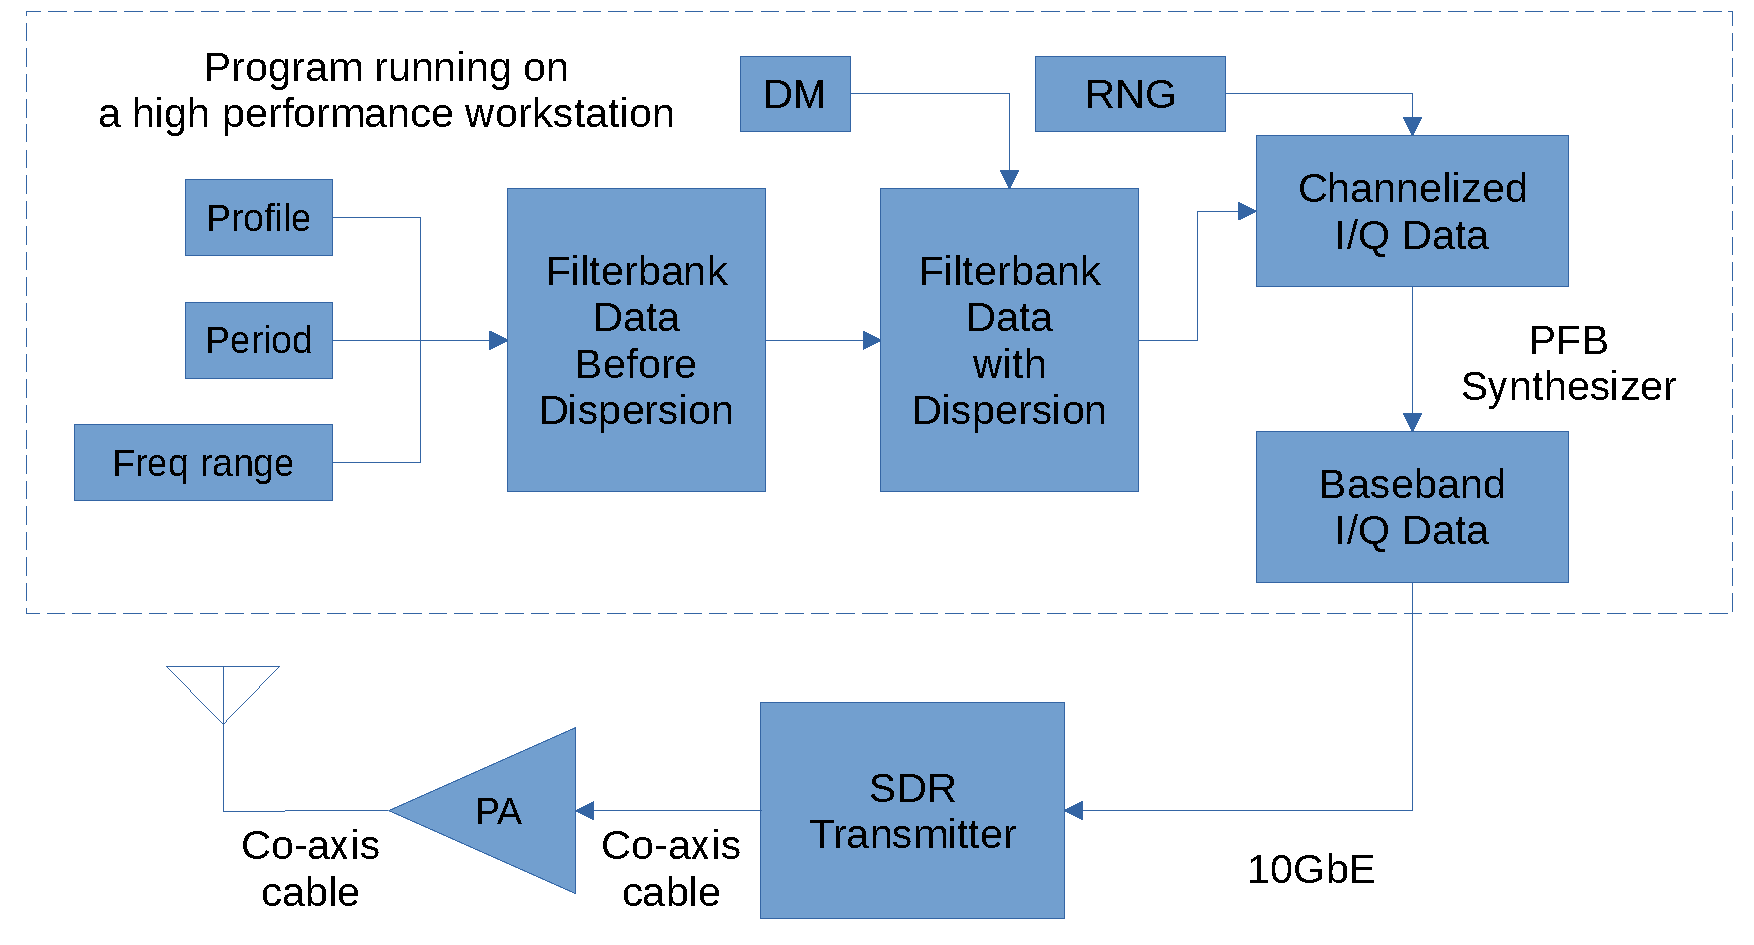
\includegraphics[width=0.95\columnwidth]{flow_chart.pdf}
    \caption{The flow chart of emitting the simulated pulsar signal.
    }
    \label{fig:flow_chart}
\end{figure}


The APD can be placed near the low-frequency pulsar observation device (LFPOD hereafter). 
Though possible, it is not necessary for the emitting antenna to be placed inside the range of the primary beam LFPOD.
The power of the emitted signal can be amplified to a high enough level so that when the signal is received by the LFPOD from its side lobes it approximates the power level of a natural pulsar.

In this section, we describe the algorithms and steps that are used to generate the radio frequency signal, which is later used to tune LFPODs.

\subsection{Computing Artificial Pulsar Signal}
\subsubsection{Generating filterbank data before dispersion}
The pulse amplitude profile $f$ is related to two variables: frequency $\nu$ and pulse phase $\theta$ and it meets
\begin{gather}
    f(\nu, \theta+1)=f(\nu, \theta)
\end{gather}
Given that the bandwidth is not extremely width, it is a good enough assumption that the frequency part and the phase part can be separated as
\begin{gather}
    f(\nu,\theta)=S(\nu)p(\theta),
\end{gather}
where $S$ is the spectrum and $p$ is the pure phase-related part.
In following sections, we simply assume $S(\nu)\equiv 1$. 
When in actual experiments, no further cost is required if we introduce a non-trivial $S(\nu)$.

By assuming 
\begin{gather}
    p(\theta)=\left \{
    \begin{array}{rl}
        p(\theta-1) &\theta \geq 0.5\\
         \exp(-\frac{\theta^2}{2w^2}) & \theta\in[-0.5, 0.5) \\
        p(\theta+1) &\theta < -0.5\\
    \end{array}
    \right ., 
\end{gather}
we calculate an example of the frequency-dependent pulse profile of a fake pulsar with period assumed to be 20 ms, as is shown in Figure \ref{fig:dm0_profile}. The frequency range is assumed to be 150-200 MHz here.

\begin{figure}
    \centering
    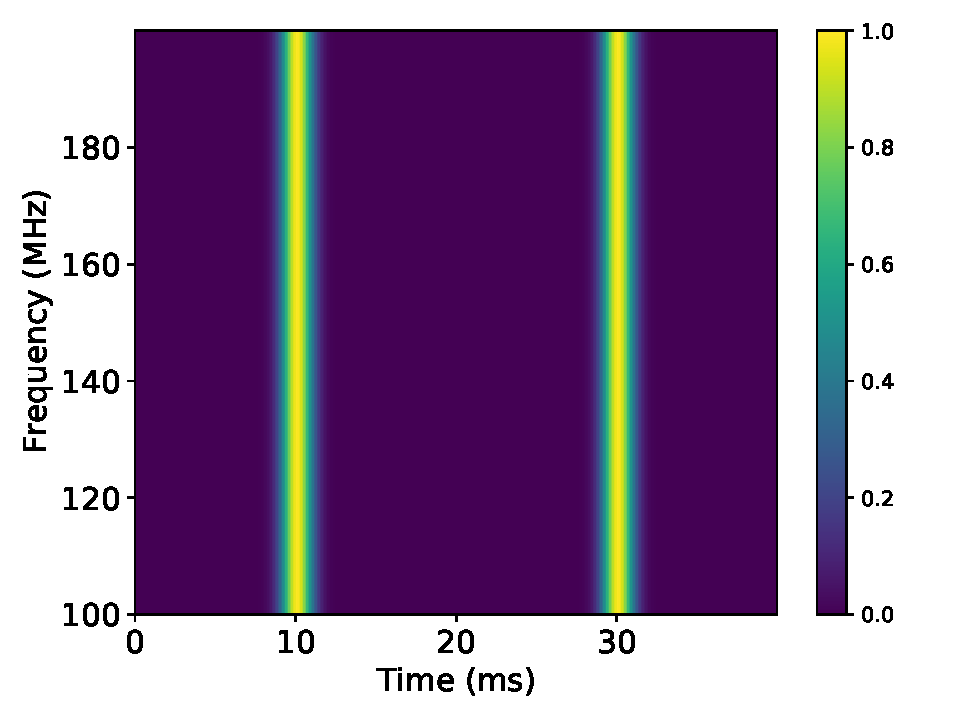
\includegraphics[width=0.9\columnwidth]{dm0_profile.pdf}
    \caption{Frequency dependent pulse profile before the dispersion effect is applied. 
    The period is set to be 20 ms and the amplitude profile is described a Gaussian function with $w=0.05$}
    \label{fig:dm0_profile}
 \end{figure}
 
 Then we need to apply the effects of dispersion to the pulse signal. According to e.g., \citet{2012hpa..book.....L}, the delay of frequency $\nu$ that is caused by the dispersion can be calculated as 
 \begin{gather}
     \Delta t(\nu)\simeq 4.15\times 10^6~{\rm ms}~\left(\frac{{\rm MHz}}{\nu}\right)^2\frac{\rm DM}{\rm pc~cm^{-3}}.
 \end{gather}
 So that the frequency dependent pulse profile after the dispersion effect is applied can be calculated as
 \begin{gather}
     f^{\rm d}(\nu, \theta)=f(\nu, \theta-\Delta t(\nu)/\tau),
 \end{gather}
where $\tau$ is the period of the pulsar. 
We show an example of frequency-dependent pulse profile after the dispersion effect is applied in Figure \ref{fig:dm10_profile}. The DM is assumed to be 10.0 and other parameters are same as what we set in Figure \ref{fig:dm0_profile}.

 \begin{figure}
    \centering
    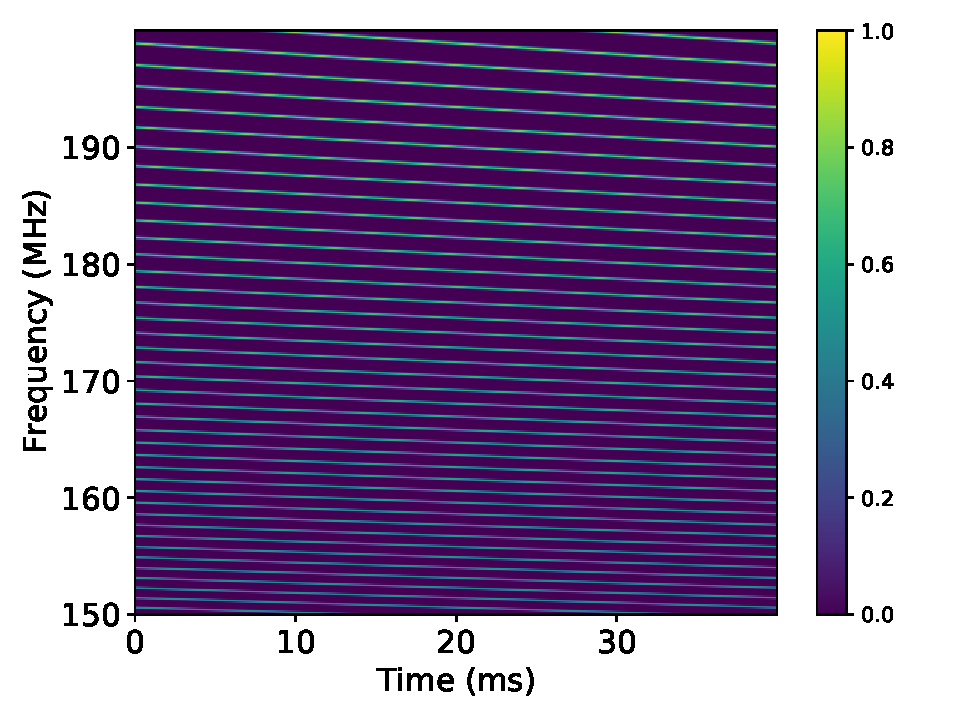
\includegraphics[width=0.9\columnwidth]{dm10_profile.pdf}
    \caption{Frequency dependent pulse profile with a $\rm DM=10$ dispersion effect applied. The parameter of the pulsar
    is same as the one used in Figure \ref{fig:dm0_profile}}
    \label{fig:dm10_profile}
 \end{figure}
 
With the amplitude profile in hand, we go on to generate the narrow band in-phase and quadrature (I/Q hereafter) signals.
First we determine the sampling interval $dt$ of the final generated I/Q time series signal and the number of frequency channels to $N_{\rm ch}$ be used in follow up procession.
The number of frequency channels further determines the bandwidth of each frequey channel as
\begin{gather}
    d\nu=\frac{f_{\max}-f_{\min}}{N_{\rm ch}}.
\end{gather}
For the sampling interval $dt$, according to the Nyquist Theorem the upper limit of which has to be $\frac{1}{2BW}$. 
For we are using I/Q sampling here the upper limit of the sampling interval is enlarged to $1/BW$.
The sampling interval of the narrow band I/Q data for current step can be calculated as
\begin{gather}
 dT=\frac{dt}{2N_{\rm ch}}.
\end{gather}
The factor 2 in the denominator is oversampling factor that we choose.
Thus the number of time bins within each period is determined 
\begin{gather}
 N_{\rm t}=\left\lfloor\frac{\tau}{dT}\right\rfloor.
\end{gather}
Note that in order to achieve a high computing performance, we limit the actual period $\tau$ can only be an integer multiple of $dT$.

So that for each frequency bin and time bin in a single period, we can calculate its instant complex voltage as
\begin{gather}
    U(\nu_{j}, t_{k})=\frac{1}{2}f^{\rm d}(\nu_j, t_{k}/\tau)(x^{\rm re}(j,k)+x^{\rm im}(j,k)i),
\end{gather}
where $j=1..N_{\rm ch}$, $k=1..N_{t}$, $i^2=-1$, and each $x^{\rm re}$ and $x^{\rm re}$ follows a standard normal distribution $\mathcal{N}(0,1)$ independently.

The narrow band I/Q data is then fed into a over-sampled polyphase filterbank (PFB) to synthesize a broadband base-band I/Q data stream.
We take the work of \citet{2020JAI.....950004M} as a reference of designing the PFB.
We set the number of channels to be $N_{\rm ch}=16384$ and the taps of each channel to be 12.
PFBs are a kind of standard digital signal processing steps, so we just skip the details of the PFB that we use in this work.

The PFB outputs the baseband I/Q sampling time series, which is then sent to an SDR transmitter so that actual radio frequency (RF) signal within desired frequency range is generated continuously.
The RF signal is fed into a power amplifier and broadcast through a proper antenna. 

\subsection{Emitting Generated Signal}

\section{An Example of Tuning}

\section{Discussion}

\section{Conclusions}

\section*{Acknowledgements}


%%%%%%%%%%%%%%%%%%%%%%%%%%%%%%%%%%%%%%%%%%%%%%%%%%

\bibliographystyle{mnras}
\bibliography{ms}

%%%%%%%%%%%%%%%%%%%%%%%%%%%%%%%%%%%%%%%%%%%%%%%%%%


% Don't change these lines
\bsp	% typesetting comment
\label{lastpage}
\end{document}

% End of ms.tex
